\documentclass[man,floatsintext]{apa6}
\usepackage[nodoi]{apacite}
\usepackage{graphicx}
\usepackage[american]{babel}
\usepackage{amsmath}
\usepackage{enumitem}
\usepackage[section]{placeins}

\title{Beyond Na\"{i}ve Cue Combination: Salience and Social Cues in Early Word Learning}
\author{Daniel Yurovsky and Michael C. Frank}
\affiliation{Department of Psychology, Stanford University}
\shorttitle{Developmental Cue Combination}
\leftheader{Yurovsky \& Frank}


\abstract{

\textbf{Research Highlights}
\vspace{-12 pt}
\begin{itemize}[noitemsep]
  \item Measured development of perceptual and social cue use in word learning
  \item Compared data to predictions of a na\"{i}ve cue-combination account
  \item Found evidence of early sensitivity to social cues
  \item Showed that developmental change was due to domain-general cognitive processes
\end{itemize}

\vspace{12 pt}

Children learn their earliest words through social \emph{interaction}, but it is unknown how much they rely on social \emph{information}. Some theories argue that word learning is fundamentally social from its outset, with even the youngest infants understanding intentions and using them to infer a social partner's target of reference. In contrast, other theories argue that early word learning is largely a perceptual process in which young children map words onto salient objects. One way of unifying these accounts is to model word learning as weighted cue-combination, in which children attend to many potential cues to reference, but only gradually learn the correct weight to assign each cue. We tested four predictions of a na\"{i}ve cue-combination account using an eye-tracking paradigm that combines social word-teaching and two-alternative forced-choice testing. None of the predictions were supported. Thus, while aspects of this unifying account are correct, it must be amended to capture both the dynamics of children's behavior across differing referential situations and general developmental changes in children's memory and attention.}

\keywords{Language acquisition, word learning, social cues, eye-tracking, cognitive development, attention}

\authornote{Please address correspondence to: 

\vspace{12 pt}
Daniel Yurovsky

Jordan Hall (Building 420)

Stanford University

450 Serra Mall

Stanford, CA 94305

\vspace{12 pt}
Email: yurovsky@stanford.edu 

\vspace{24 pt}

Word Count: 6030
}

\begin{document}
\maketitle


How do children learn the meanings of their first words? A number of influential theories conceptualize young infants' primary learning mechanism as making associations between perceptual stimuli \cite{Piaget1952, Vygotsky1978}. On these kinds of accounts, infants learn the meanings of labels like ``ball'' and ``dog'' by mapping them onto salient objects in their learning environments \cite{Werker1998,Smith2000}. These accounts are appealing on grounds of parsimony: The mechanisms they require for the onset of word learning---perceptual orienting and associative mapping---are universally agreed to be in the repertoire of young infants (\citeNP<e.g.>{Fantz1964,Haith1980}; although \citeNP<c.f.>{Spelke1998}). In addition, the ecological context of language learning appears to support perceptually-driven learning. For instance, early child-directed naming events are characterized by multi-modal synchrony: mothers move the objects they label in temporal synchrony with the labels they speak \cite{Gogate2000}, and the degree of synchrony predicts successful word-object mapping for young infants \cite{Gogate2006}.\footnote{For convenience here---and reflecting the orientation of our work towards concrete noun learning---we refer to ``word-object mapping'' and ``word learning'' interchangeably. Of course, mapping is only a small part of the process of learning a word, which includes at least: learning a phonological form, mapping this form to a referent, inferring the meaning that licenses this reference and how it generalizes across instances, and retaining all of this information in memory for future use.}

Infants are also situated in a social system from their first day of life, however. This social system is the \emph{source} of the multi-modal structures in their perceptual input. Alternative theories of word learning thus argue that infants leverage social---not just perceptual---information when learning even their first words \cite{Bruner1983,Bloom1998}. For instance, infants follow direction of gaze by 6-months \cite{Dentremont1997}, especially in the presence of other communicative signals \cite{Senju2008}. Further, individual differences in gaze-following predict differences in vocabulary development \cite{Brooks2008}. In addition, in some experiments infants appear to be representing others' communicative goals, and these representations affect their expectations about language by 12 or even 6 months of age (\citeNP{Vouloumanos2012, Vouloumanos2014}). Infants are thus tuned to social cues, and could in principle already use these cues from the outset of word learning.

Because these two classes of theories---perceptual and social---are posed as mutually-exclusive competitors, and because both are supported by compelling empirical findings, each has attempted to re-conceptualize the evidence in favor of the other in its own terms. For example, researchers in the perceptual tradition have shown that cases of putatively social understanding can be explained as a set of learned perceptual associations \cite<e.g.>{Goldstein2008, Yu2012c, Deak2014}. On the other side, researchers from the social tradition have argued that the perceptual signals shown to drive learning are effective \emph{because} infants infer that they are being presented by a social, pedagogically motivated caregiver \cite{Csibra2010, Deligianni2011}. 

Unifying these two accounts within a single framework provides a promising theoretical alternative. As advocates of social word learning point out, children must learn more than mappings between labels and objects in the world. While object labels represent a large slice of typical early vocabularies \cite{Caselli1995,Tardif2008}, young children also learn verbs, adjectives, and many other word types \cite{Fenson1994,Clark2003,Bergelson2013}. It is likely that the kinds of mechanisms advanced in perceptual accounts of early word learning are not completely sufficient to explain this diversity of word meanings \cite{Gleitman1990,Bloom2000,Waxman2009}, despite work showing that these mechanisms do play a role \cite{Piantadosi2012,Scott2012}. While we focus here on concrete noun learning, the scalability of learning mechanisms to the broader vocabulary is an important theoretical concern for unifying models.

One possible proposal for unification is that infants are sensitive to many cues to reference: both perceptual cues like visual salience and temporal contiguity \emph{and} social cues like eye-gaze and pointing. To determine the referent of a speaker's utterance, children could combine all of the available cues, assigning each a weight proportional to its predictive validity. On such an account, developmental changes in determining a speaker's target of reference are due to a process of learning the correct weights to assign to each kind of cue. Early on, children may be biased to assign high weight to perceptual cues. However, over development, children might gradually assign higher weight to social cues as they learn that they are powerful predictors of a speaker's referential intentions. Similarly, children might reduce the weight they assign to perceptual cues as they discover that they are ineffective predictors of referential intention \cite{Hollich2000, Golinkoff2006}. The goal of the current work is to test this kind of unifying ``developmental cue combination'' account; we begin by reviewing previous research supporting such an account and then derive several predictions, which we test in two experiments. 

\subsection{Data Supporting Developmental Cue Combination}

The primary support for a developmental cue-combination account comes from studies that pit perceptual salience against social information (e.g., speaker gaze) and measure children's learning under these conditions at different ages. \citeA{Hollich2000} presented 12 studies that varied the referential cues highlighting two different objects in ambiguous naming events. In the first three experiments, one of the objects was perceptually salient, and one was fixated by the speaker. Analyses compared a condition in which the same object received both cues (Coincidental) to a condition in which the cues pointed to different objects (Conflict). In these studies, 19- and 24-month-olds appeared to assign more weight to the social cue, preferentially mapping the label onto the object the speaker fixated regardless of which was more salient. In contrast, although 12-month-olds showed some evidence of following the speaker's gaze in training, they looked more at the more salient object at test in both conditions. A followup experiment from \citeA{Pruden2006} showed that 10-month olds did not attend to the speaker's gaze at all.

In almost all of these studies, however, target and competitor objects remained in the same position during both training and test. Thus, it is unclear whether infants in these studies mapped the label onto an object or onto a location \cite<e.g.,>{Benitez2012}. In the two experiments in which target position switched from training to test, learning was disrupted for all of the age groups except the 24-month-olds \cite{Hollich2000, Pruden2006}. This finding is consonant with earlier data  showing in a head-turn procedure that conflicting perceptual and social cues disrupted learning in 18- but not 24-month-olds \cite{Moore1999}. 

Together, these studies present data that are supportive of a developmental cue combination account, but nevertheless leave several questions unresolved. First, these studies present an incomplete picture of children's behavior in learning trials. While they describe children's preferential looking at one object over the other, they miss a third critical component of these naming events: the attention to the speaker. While children's use of perceptual cues can be inferred straightforwardly from looks to the objects, characterizing their uptake of social cues requires measuring their engagement with the speaker. Second, it is unclear from prior work whether changes in the relative strengths of social and perceptual cues would be due to increasing weights for social cues, decreasing weights for perceptual cues, or both. Answering this question would require comparing conditions where cues are in opposition to a condition where \emph{only} the social cue is available.\footnote{While \citeA{Moore1999} did compare these conditions, they have relatively low power to detect differences between them due to small samples and a challenging test measure (forced choice responding). \citeA{Hollich2000} ran studies using gaze alone with 12-month-olds, but not with older age groups.} The goal of our current studies is thus to gather a large, developmentally-broad eye-tracking dataset on children's behavior in cue-combination tasks, both during training and at test. This dataset allows us to make a direct test of predictions of the developmental cue combination account, which in turn addresses these questions.

\subsection{Testing Predictions of Developmental Cue Combination: The Current Study}

Weighted cue-combination is an intuitive, computationally simple model of the process of change in early word learning. For example, a number of computational models have implemented a version of this idea  \cite{Frank2007b,Yu2007b,Frank2013a}. Developmental cue combination is also consistent with properties of our perceptual system: Within and across modalities, adults weigh cues in proportion to their predictive power, combining them as predicted by ideal observer models \cite{Ernst2002, Jacobs2002}. Despite this intuitive plausibility, a number of detailed predictions of cue combination models remain untested, specifically as they apply to these models as a description of developmental change in children's concrete noun learning. 

In the current study, we test four predictions of the cue-combination model of developmental change:

\begin{enumerate}[noitemsep]
	\item Developmental change is due to re-weighting across cues,
	\item Perceptual cues decrease in weight across early development, 
        \item Social cues increase in weight across early development, and
	\item Cue weights drive attention during learning.
\end{enumerate}

\noindent Prediction \#1 is derived directly from previous work on the ECM model, which has suggested that a major developmental change during the second year was a move from reliance on salience to reliance on social cues \cite{Hollich2000,Golinkoff2006}. The developmental cue combination account predicts that this shift should be a major driver of developmental change in word learning during this period. Predictions \#2 and \#3 are corollaries of Prediction \#1, again following from previous work that suggested that perceptual cues were less relevant for older children, whose learning was informed more by social cues. Finally, Prediction \#4 comes from the idea that cue combination affects learning through the biasing of attention; thus, greater cue weights on social cues relative to salience should be reflected by shifts in the distribution of gaze when these two cues are in conflict. 

In two experiments, we show that none of these predictions are supported. Thus, while cue-combination captures important insights about early word learning, a na\"{i}ve version of this account is insufficient to explain the observed developmental trajectory. We end by discussing possible modifications to this view.

\section{Experiment 1}

In nearly all previous experiments investigating cue-combination in early word learning, social cues were pitted against perceptual cues \cite<c.f.>{Moore1999}. Thus, results indicating developing preferences for social information over perceptual information are consistent with three possible explanations: (1) social cues increase in weight, (2) perceptual cues decrease in weight, or (3) perceptual and social cues both change in their \emph{relative} weight. Experiment 1 was designed to distinguish between these three possibilities by independently measuring the development of children's abilities both to follow and to learn from social gaze, \emph{in the absence of competing salience cues}. A na\"{i}ve cue-combination account, in which developmental changes in cue use result from learning their relative predictive weights, makes a null prediction: Children's responses should not change significantly across development when only one cue is available. 

We tracked children's eye movements while they watched a series of naturalistic word-learning videos. In each, children saw a speaker seated at a table between two novel toys. She greeted them, and then turned towards one of the toys and labeled it three times in a short monologue. After these learning trials, children were tested for their knowledge of the referent for the new word using the preferential looking procedure. In addition, to measure children's processing abilities for familiar words, they were also tested in preferential looking trials with two known items. In Experiment 1, the two novel toys were chosen to be equally salient to children (see Appendix).

\subsection{Method}

\begin{figure}[tb]
	\center{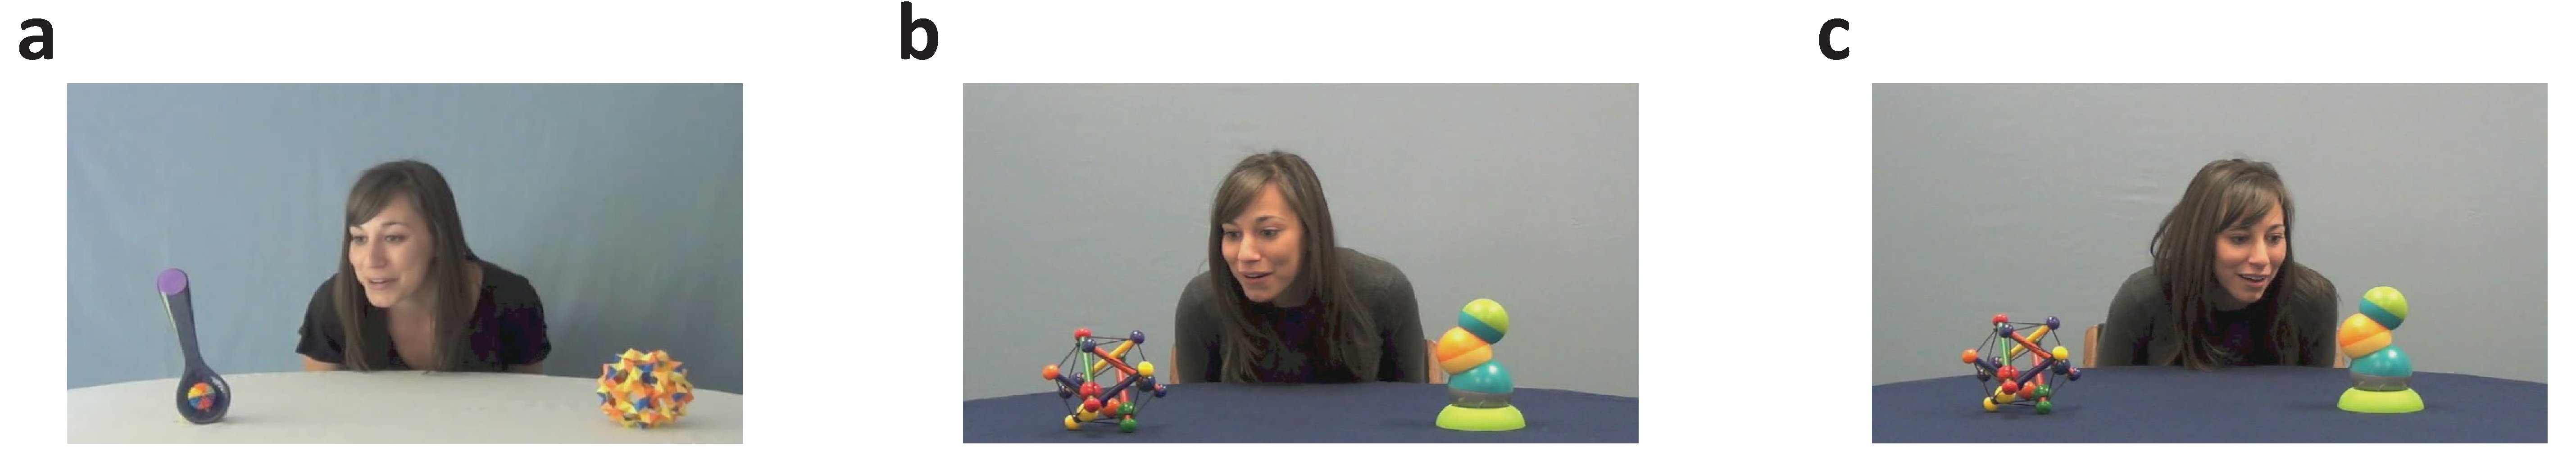
\includegraphics[width=\textwidth]{figures/tri_fig.pdf}}
	\caption{\label{fig:design} Example learning trials from Experiments 1 and 2. In Experiment 1 (a), the speaker turned towards one of the equally-salient toys and labeled it three times over the course of $\sim$12s. In Experiment 2, the speaker produced the same social cues and the same label as in Experiment 1, but the target object was either the more perceptually salient toy (b), or the less perceptually salient toy (c). These manipulations allowed us to measure the contributions of both salience and social information to word-object mapping.}
\end{figure}

\subsubsection{Participants}

Parents and their 1--4 year-old children were invited to participate in a short language learning study during their visit to the San Jose Children's Discovery Museum. In total, we collected demographic and experimental data from 269 children, 122 of whom were excluded for one or more of the following reasons: self-reported developmental issues (e.g., autism, language delays, etc.; $N= 27$), failure to calibrate ($N=58$), and less than 75\% exposure to English ($N=36$).\footnote{These exclusion criteria were preset in this study on the basis of previous work \cite{Yurovsky2013c}. Our high exclusion rate is due to inclusive recruitment, congruent with the outreach component of recruiting in a museum context.} The final sample consisted of 27 1--1.5 year olds (9 girls), 19 1.5--2 year olds (7 girls), 38 2--2.5 year olds (13 girls), 26 2.5--3 year olds (10 girls), 15 4--3.5 year olds (9 girls), and 22 3.5--4 year olds (11 girls).

\subsubsection{Stimuli and Design}

The experiment consisted of two kinds of trials designed to measure both how children allocate their attention while learning from a social partner, and what word-object mapping information they extract from these learning events. Learning trials were $\sim$12s video clips in which a speaker first greeted the the child, and then turned towards one of the two toys on the screen, labeling it three times in a short monologue (Figure~\ref{fig:design}a). On the first learning trial, for example, the speaker said ``Hi there! It's a \emph{modi}. Look at the \emph{modi}. What a nice \emph{modi}.''

On each test trial, children saw two objects---one on each side of the screen---and heard a short audio clip of the speaker from the learning trials asking them to find a target object. Each test trial was 7s long, and the target label was heard at ~2.75s. On \emph{Familiar} test trials, both the target and competitor were common objects familiar to young children (e.g. book vs. dog). On \emph{Novel} and  \emph{Mutual Exclusivity (ME)} test trials, children saw both of the toys from the previous learning trials, and were asked to find either the previously named toy (\emph{modi}), or were asked to find the target of a novel label (\emph{dax}). These ME trials were designed as a strong test of mapping formation. Looking to the correct target on Novel trials alone could result from familiarity or preference rather than mapping, but correct performance on both Novel and ME trials could only result from knowledge of the specific label used during the learning phase.


\subsubsection{Procedure}

We collected eye-movement data with an SMI RED corneal-reflection eye-tracker mounted on an LCD monitor, sampling at 120Hz. The eye-tracker was first calibrated for each child using a 2-point calibration. Next, children saw four learning trials in which the speaker looked at one of two toys on the screen and labeled it three times. Finally, children saw the test trials, in which their knowledge of both familiar and novel word-object mappings was tested. The entire experiment consisted of 4 learning trials, 8 Familiar, 6 Novel, and 6 ME test trials. We additionally inserted two calibration checks: short videos in which small dancing stars appeared in four places on the screen.  These checks allowed us to adjust initial calibration settings when they were imprecise (see below).

\subsection{Results and Discussion}

We analyzed children's eye movements using a Region of Interest (ROI) approach. Bounding-box ROIs were drawn by a human coder for the speaker's face (learning trials) and for the two objects (learning and test trials). Children's learning and test behaviors were quantified by measuring their proportion of looking to each ROI on each trial. To ensure that proportions were representative, individual test trials were excluded from analysis if eye gaze data were missing for more than half of their duration. To compute age-group looking proportions, proportions were computed first for each individual trial, averaged at the individual-child level, and then averaged across children. To ensure accuracy in our identification of point of gaze, children's calibrations were adjusted by fitting a robust linear regression for their fixations relative to known locations on calibration check videos. These regressions were used to correct the calibration of eye movements for all learning and test trials \cite{Frank2012d}.

We begin by describing children's behavior during both learning and test trials, then we present statistical analyses, and finally discuss implications for the predictions of the developmental cue combination model. 

\subsubsection{Descriptive Analyses}

First, children in all age groups spent the majority of learning trials fixating the speakers face, although this proportion decreased across development. Interestingly, looking to the face remained relatively constant over the course of the naming events (Figure~\ref{fig:exp1_train_spaghetti}). Similarly, the second most-fixated ROI at all ages was the target object. Proportion of looks to the Target increased across early development, and like Face-looks, remained relatively constant over the naming event. Looking to the competitor was consistently low at all ages. Thus, across development, children appeared to attend to the speaker, and follow her gaze to the target object over the competing object. The major developmental change during the learning phase appeared to be improvement in the ability to disengage from the speaker.

\begin{figure}[tb]
	\center{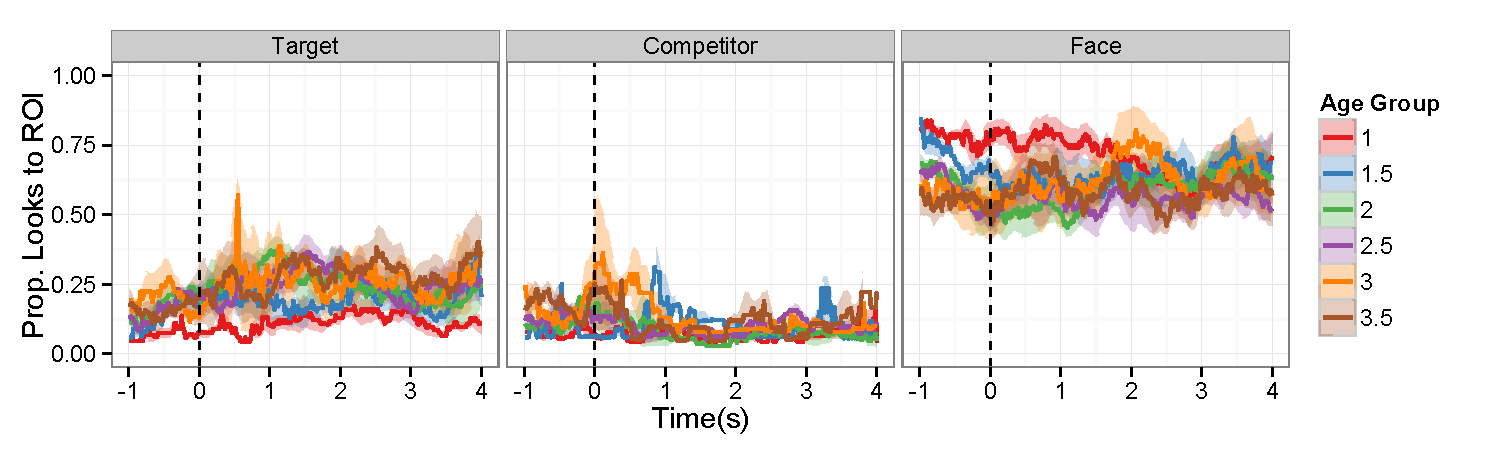
\includegraphics[width=\textwidth]{figures/exp1_train_spaghetti.pdf}}
	\caption{\label{fig:exp1_train_spaghetti} Looking behavior during learning trials in Experiment 1. Children in all age groups spent the majority of naming events looking at the speakers face, but looking to the face decreased and looking to the target increased across development. Looking to the competitor stayed constant. Each curve represents an age-group mean, and shaded regions indicate $\pm$1 SE. For clarity, curves were smoothed by taking the average within a 60ms moving window.}
\end{figure}

At test, children at all ages were able to find the target referents of known words on Familiar trials. Both speed and accuracy improved across development, and additionally the 3 and 3.5 year olds attended to the target for longer, rebounding after checking back to the competitor (Figure~\ref{fig:exp1_test_spaghetti}). Looking patterns were broadly similar on Novel trials, although overall accuracy was lower and the youngest age groups appeared to find the target more slowly. Mutual Exclusivity trial performance also showed similar trends, although there was little evidence that the youngest children---1-1.5 year olds---were correctly looking at the previously un-named object on ME trials (consistent with prior work on mutual exclusivity with this age group; \citeNP{Halberda2006}).

\begin{figure}[tb]
	\center{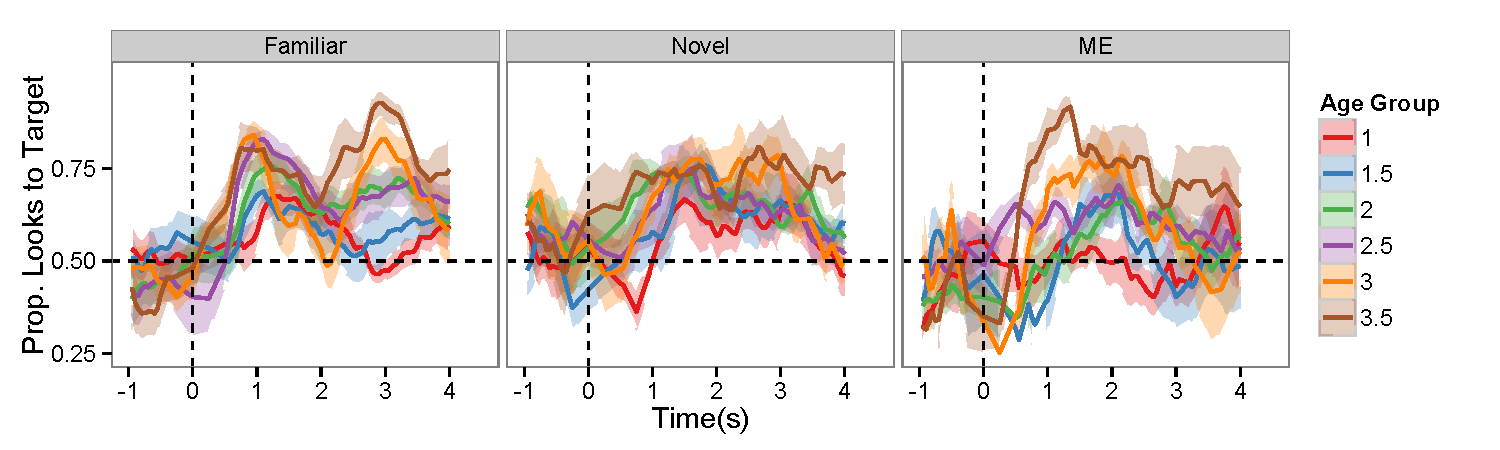
\includegraphics[width=\textwidth]{figures/exp1_test_spaghetti.pdf}}
	\caption{\label{fig:exp1_test_spaghetti}Looking behavior at test in Experiment 1. Children improved in both speed and accuracy on all three trial types---Familiar, Novel, ME---across development. Plotting conventions are consistent with Figure~\ref{fig:exp1_train_spaghetti}.}
\end{figure}

A clearer way of seeing these trends is through onset-contingent analyses \cite{fernald2008}. Figure~\ref{fig:exp1_split} shows the same data split by the object that was the focus of attention at the onset of the label. In each panel, the two lines show the proportion of children over time who switched to look at other object if they---by chance---began the trial on the target (solid), or competitor (dotted). If children knew the correct referent on a trial and looked at it, those who began on the competitor should have switched to the target, and those who began on the target should have remained on the target. The area between these two curves is informative about the strength of children's discrimination of target vs. distractor, and the time point at which curves diverge is informative about the speed with which the discrimination was made. In addition, these trajectories can be informative about the processes underlying this discrimination \cite{Halberda2006}. 

These graphs show broad improvement both in speed and accuracy across development; the area between the two lines in each curve is larger, and the point of divergence between the two curves is earlier. They also showcase the difference in difficulty between Novel and Mutual Exclusivity trials. The two ME curves for one-year olds overlap for essentially the entire duration of test trials; for 1.5-year-olds, the dotted line is above the solid line (indicating fixation to the correct object) for only a short window of time in the middle of the trial. 

\begin{figure}[tb]
	\center{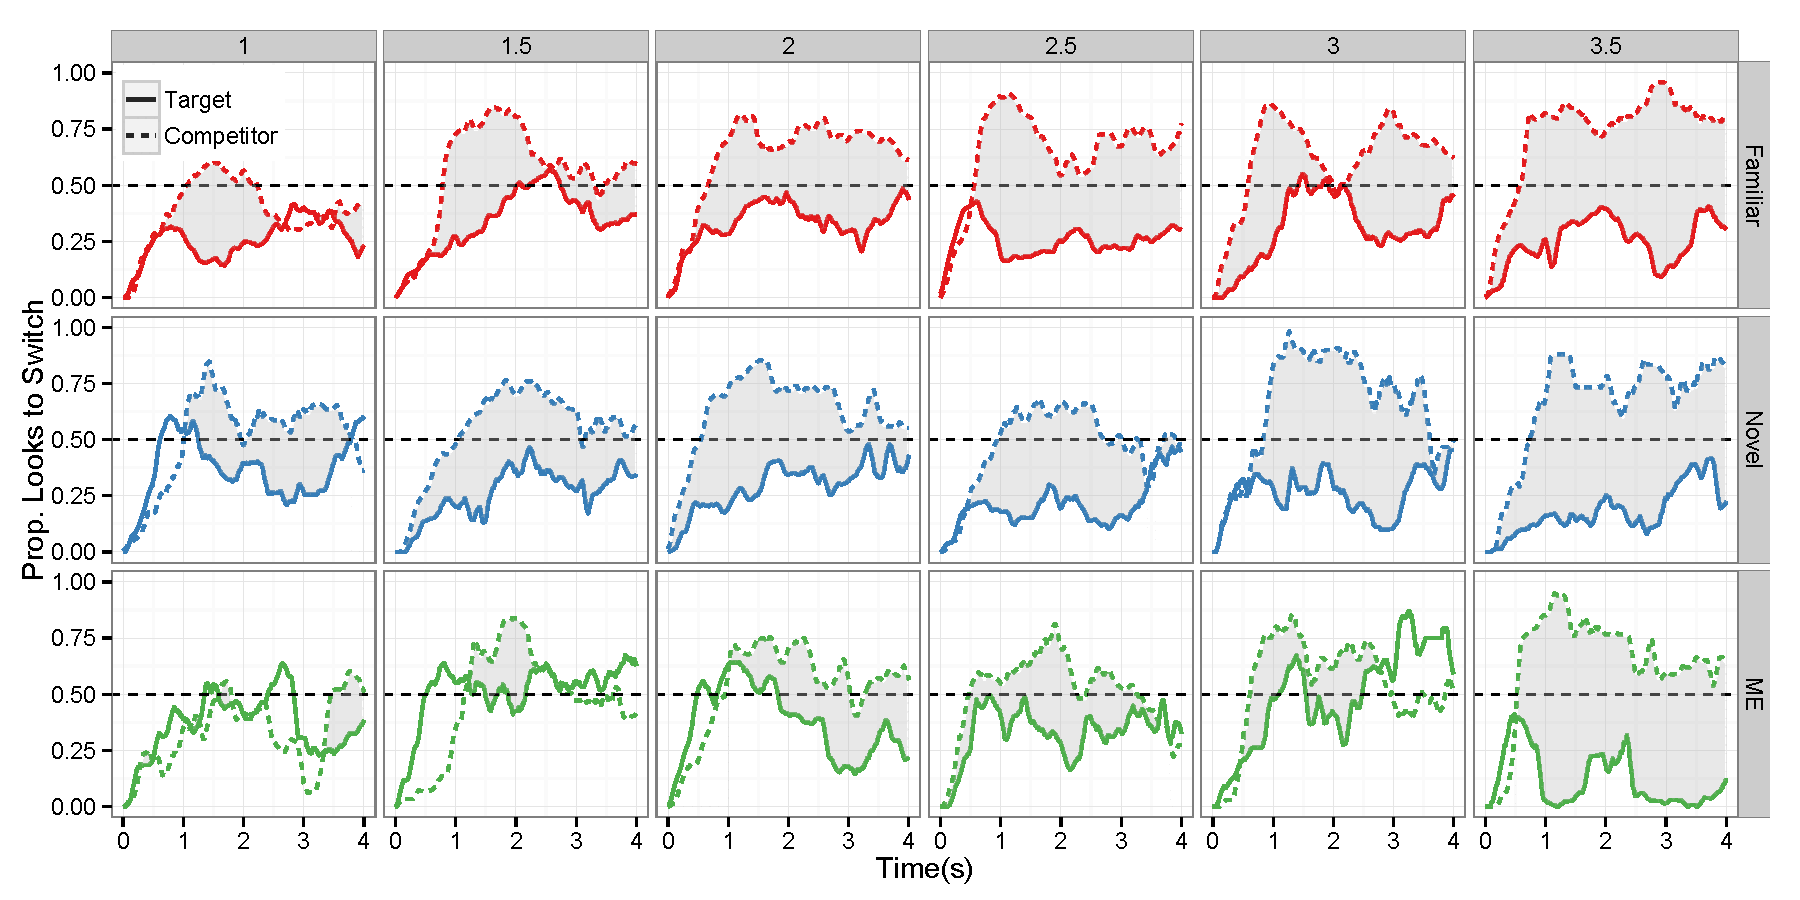
\includegraphics[width=\textwidth]{figures/exp1_split_plot.pdf}}
	\caption{\label{fig:exp1_split} Onset-contingent plots for test trials in Experiment 1. Each panel shows the proportion that shifted from one referent to the other across time. The solid line represents children who (by chance) began the trial on the correct target, and the dotted line represents children who began on the competitor. The size of the gray shaded region---the region where more switches were made from competitor-to-target than from target-to-competitor---is indicative of how much children discriminated between the two toys in the context of the label.}
\end{figure}

Together, these descriptive analyses suggest that from the earliest age we measured, children were engaged in the naming events and followed the speaker to the target of her reference using the direction of her head and gaze. Across development, children became better able to disengage from the speaker and spent more time looking at the target. In addition, speed and accuracy on all three test types (Familiar, Novel, and ME) improved across development. To quantify these impressions with standard measures, we aggregated over these time-course measures to compute proportion of looking in a particular temporal window of interest. These windows began at the point of disambiguation for each trial. For test trials, the point of disambiguation was the onset of the target label, and for learning trials it was the rotation of the speaker's head. The window for each trial began 1s after this point of disambiguation to allow children of all ages enough time to process and continued out to 3s after this point on both learning and test trials. To quantify learning using standard statistical analyses, we aggregated dwell-time in ROIs within temporal windows to compute the proportion of looking at each location on each trial.

\subsubsection{Statistical Analyses}

 \begin{figure}[tb]
	\center{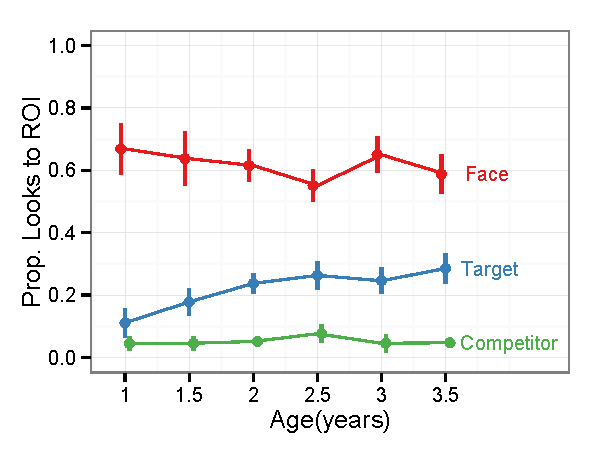
\includegraphics[width=.65\textwidth]{figures/exp1_train.pdf}}
	\caption{\label{fig:exp1_train} Proportion of children's looking the target toy, competitor toy, and the speaker's face during learning trials in Experiment 1, summarizing the developmental trends shown in Figure \ref{fig:exp1_train_spaghetti}. Children of all ages spent the majority of the learning trials looking at the speaker's face. Disengaging from the face and fixating the target increased across development. Error bars indicate 95\% confidence interval computed by non-parametric bootstrap.}
\end{figure}

Inspection of time course plots showed that children in all age groups were successful at attending to and following the speaker's social gaze during learning trials at all ages. Statistical analysis confirmed this impression: children of all ages spent more time looking at the target than at the competitor during learning trials (smallest $t(23)  = 3.20$, $p < .01$, $d =.65$) ; Figure~\ref{fig:exp1_train_test}). However, for all age groups, looks to both target and competitor made up the minority of children's dwell times. Instead, children in all age groups spent more than 50\% of their time attending to the speaker's face (Figure~\ref{fig:exp1_train}).\footnote{All data and code for analysis available at \small{\tt{http://github.com/dyurovsky/ATT-WORD}}.} 

\begin{figure}[tb]
	\center{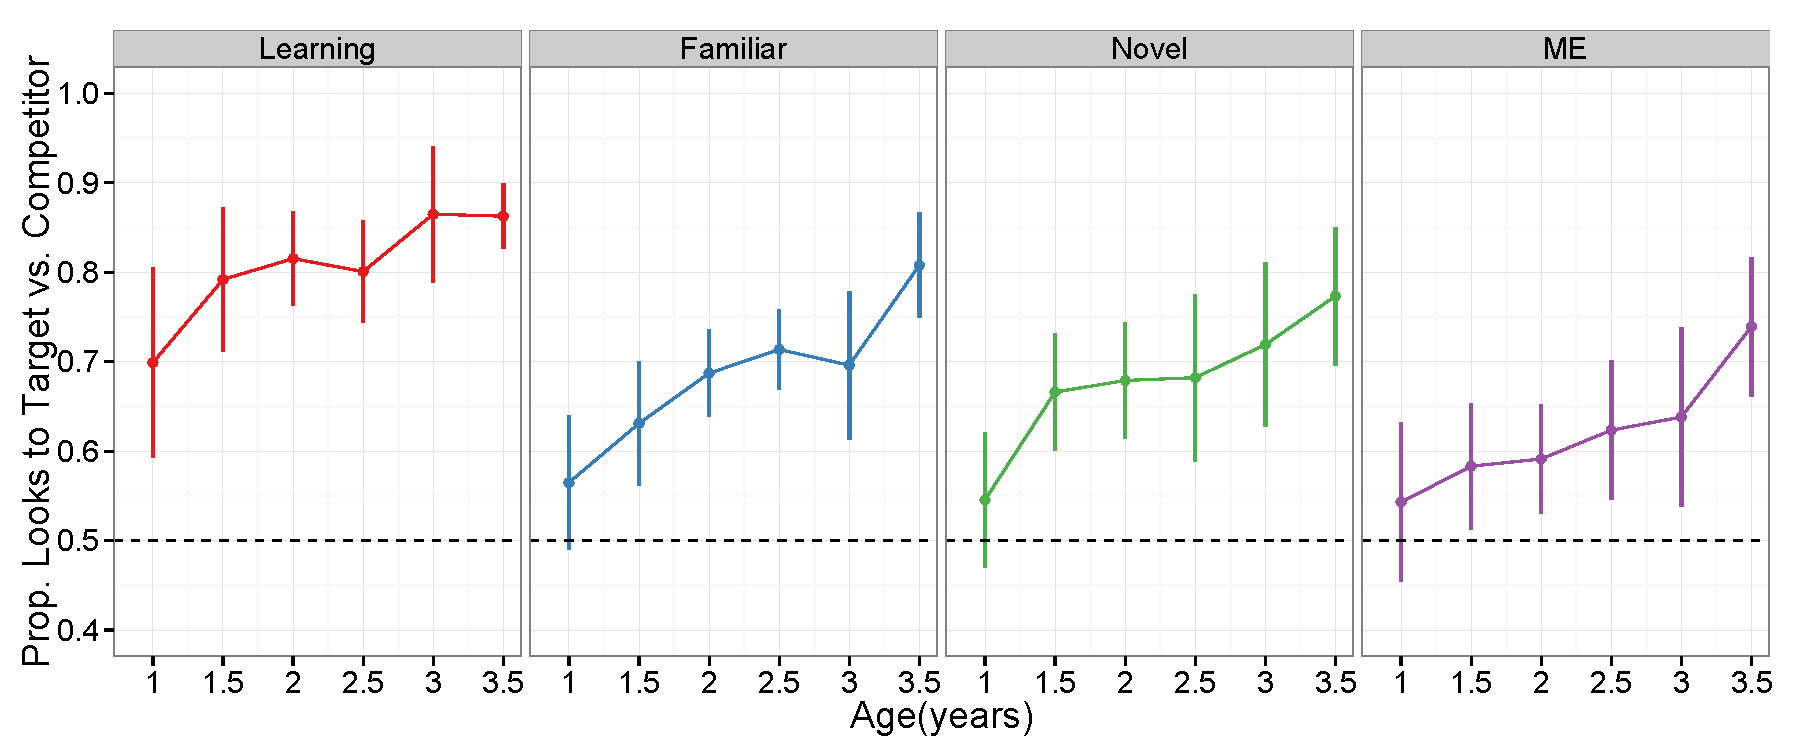
\includegraphics[width=\textwidth]{figures/exp1_train_test.pdf}}
	\caption{\label{fig:exp1_train_test} Proportion of time children fixated the correct target on each trial type in Experiment 1. Children improved on all measures across development. Each dot indicates one half-year age group and each line represents a 95\% confidence interval computed by non-parametric bootstrap. A proportion of .5 indicates chance performance.}
\end{figure}	

Similar analyses of test trials showed broad success on Familiar, Novel, and ME trials across development. The 1--1.5 year-olds trended towards significance on Familiar trials ($t(26)  = 1.65$, $p = .11$, $d = .32$), and were non-significantly in the correct direction on Novel and ME trials. At all other ages, children looked to the target at above-chance levels on all test trials (smallest $t(17)  = 2.10$, $p = .05$, $d = 1.16$). These analyses are consistent with previous work showing the emergence of success on ME trials from approximately 16-18 months \cite<e.g.>{Halberda2006, Bion2013}.

To quantify the change we observed across development, we fit a mixed effects logistic regression to the proportion of looking data during both learning and test \cite{Jaeger2008}. Our regression model predicted the proportion of looking to the target on each trial using and trial type (Learning, Familiar, Novel, ME) with Novel as the reference trial type. To make data from the learning phase comparable with those from the test phase, we computed the proportion looking to the target vs. the competitor object, excluding looks to the face.  This analysis revealed significant improvements in target looking across age ($\beta = .61$, $z = 4.03$, $p <.001$), as well as a significant effect of Learning as compared to Novel trials ($\beta = 1.18$, $z = 3.11$, $p <.01$). No other trial types were significantly different from the Novel baseline, and a model with an interaction between age and trial type was not a significantly better fit to the data. These statistical analyses together suggest that children were more successful at finding the correct target during learning trials, but that they improved similarly on all trial types across development, capturing the general developmental trends shown in Figure \ref{fig:exp1_train_test}.

\subsubsection{Summary}

Together, these results provide evidence both of early competence in the use of social gaze to determine the target of a speaker's reference, as well as improvement in this skill across development. Further, improvements in gaze-following also paralleled improvements in both finding the referents of novel words on subsequent test trials, and also finding the referents of familiar words.

How well do these results fit with the developmental cue combination account? First, there was no conflict between cues in this experiment, so any changes observed in behavior could not be due to \emph{relative} reweighing of cues (Prediction \#1). Thus, this prediction is not supported. One way around this conclusion would be to argue that what we observed was developmental change in \emph{absolute} weight for social information. But such a description seems to be at best a misleading account of the data: Performance on familiar word recognition trials appeared to be changing at roughly the same rate as recognition of novel words. This congruence suggests that a parsimonious account of development would be general changes in speed of word recognition \cite<e.g.>{fernald1998,Fernald2006a}, not changes in social cue weight, which after all would be irrelevant for familiar word recognition.

Second, these results also speak against Prediction \#4 of the cue combination account, that cue weights drive attention during learning. Children at all ages found the speaker's face highly engaging, and spent the majority of their time fixating it, rather than the referents on learning trials. The primary behavioral development we observed was the ability to {\it disengage} from the speaker's face. This result is congruent with findings from 1--2 year-olds suggesting developmental increases in the ability to disengage from faces in favor of other targets \cite{Frank2012d}. Disengagement in our stimuli was due to gaze-following---and hence relevant to the use of social information---but in some sense this behavior is the opposite of what the cue combination account predicts. The less children's attention is captured by particular social stimuli, the more they are free to attend flexibly to aspects of the context that may be relevant for understanding. 

In sum, data from Experiment 1 did not support the predictions of the developmental cue combination account. Instead, the developmental trends we observed appeared more consistent with a different account. In our data, developmental changes appeared to be driven by changes in general processes of attention and memory combined with increasing familiarity with and fluency in processing spoken language. Nevertheless, the primary data of interest for earlier tests of cue combination were conflicts between cues \cite{Hollich2000}, so to fully test these theories it is important to investigate such conflicts. In Experiment 2 we manipulated the relative salience of the target and competitor objects during learning trials with gaze cues. This manipulation allowed us to measure how salience affects children's looking during both learning and test.

\section{Experiment 2}

Experiment 2 was identical to Experiment 1 in all respects except for the identity of the novel toys that served as the target and competitor. In contrast to Experiment 1, in which the two toys were balanced in their visual salience, the two toys in Experiment 2 were mismatched (see Appendix). For children in the \emph{Salient} condition, the target was the more interesting toy, and the competitor the less interesting toy. In the \emph{NonSalient} condition, the identities of the toys were switched---the target was the less salient toy. Experiment 2 thus allowed us to investigate children's use of social cues to learn new words when both social cues and salience indicate the same referent, and when they are in competition \cite<as in>{Hollich2000,Pruden2006}.

\subsection{Method}

\subsubsection{Participants}

Participants were recruited from the floor of the San Jose Children's Discovery museum as in Experiment 1. For Experiment 2, we focused on the three youngest age groups. In the Salient condition, demographic and experimental data were collected from 117 children, 52 of whom were excluded for one or more of the following reasons: developmental issues ($N= 13$), failure to calibrate ($N=25$), less than 75\% exposure to English ($N=33$), and inattentiveness ($N=2$). The final sample consisted of 22 1-1.5 year olds (11 girls), 21 1.5-2 year olds (10 girls), 19 2-2.5 year olds (9 girls). 

In the NonSalient condition, data were collected from 126 children, 71 of whom were excluded for one or more of the following reasons: developmental issues ($N= 9$), failure to calibrate ($N=26$), and less than 75\% exposure to English ($N=36$). The final sample consisted of 26 1-1.5 year olds (13 girls), 25 1.5-2 year olds (11 girls), 15 2-2.5 year olds (4 girls).

\subsubsection{Stimuli, Design, and Procedure}

Experimental stimuli were identical to those in Experiment 1, except that the identities of the novel toys were changed and new videos were recorded. The procedure, including the order of the trials, was identical.

\subsection{Results and Discussion}

To determine the effect of perceptual salience on word learning, we compared children's looking in the Salient and NonSalient conditions not only to each other, but also to the Balanced condition tested in Experiment 1. As before, we begin by presenting basic descriptive analyses, then statistical analyses, and finally a summary of implications for the na\"{i}ve cue combination account of early word learning.

\subsubsection{Descriptive Analyses}

As in Experiment 1, children spent the majority of learning trials looking at the speaker's face, and this proportion remained relatively constant over the course of the naming event. Further, children again successfully followed the speaker to the correct target---both when it was the Salient toy and when it was the NonSalient toy---in all three age groups. Figure~\ref{fig:exp1and2_train_spaghetti} shows the data from the Salient and NonSalient conditions alongside data from the Balanced condition of Experiment 1. Looking behavior across all three conditions (rows) appears strikingly similar, showing very little effect of perceptual salience during learning trials. We return to this observation in the statistical analyses below.

\begin{figure}[tb]
	\center{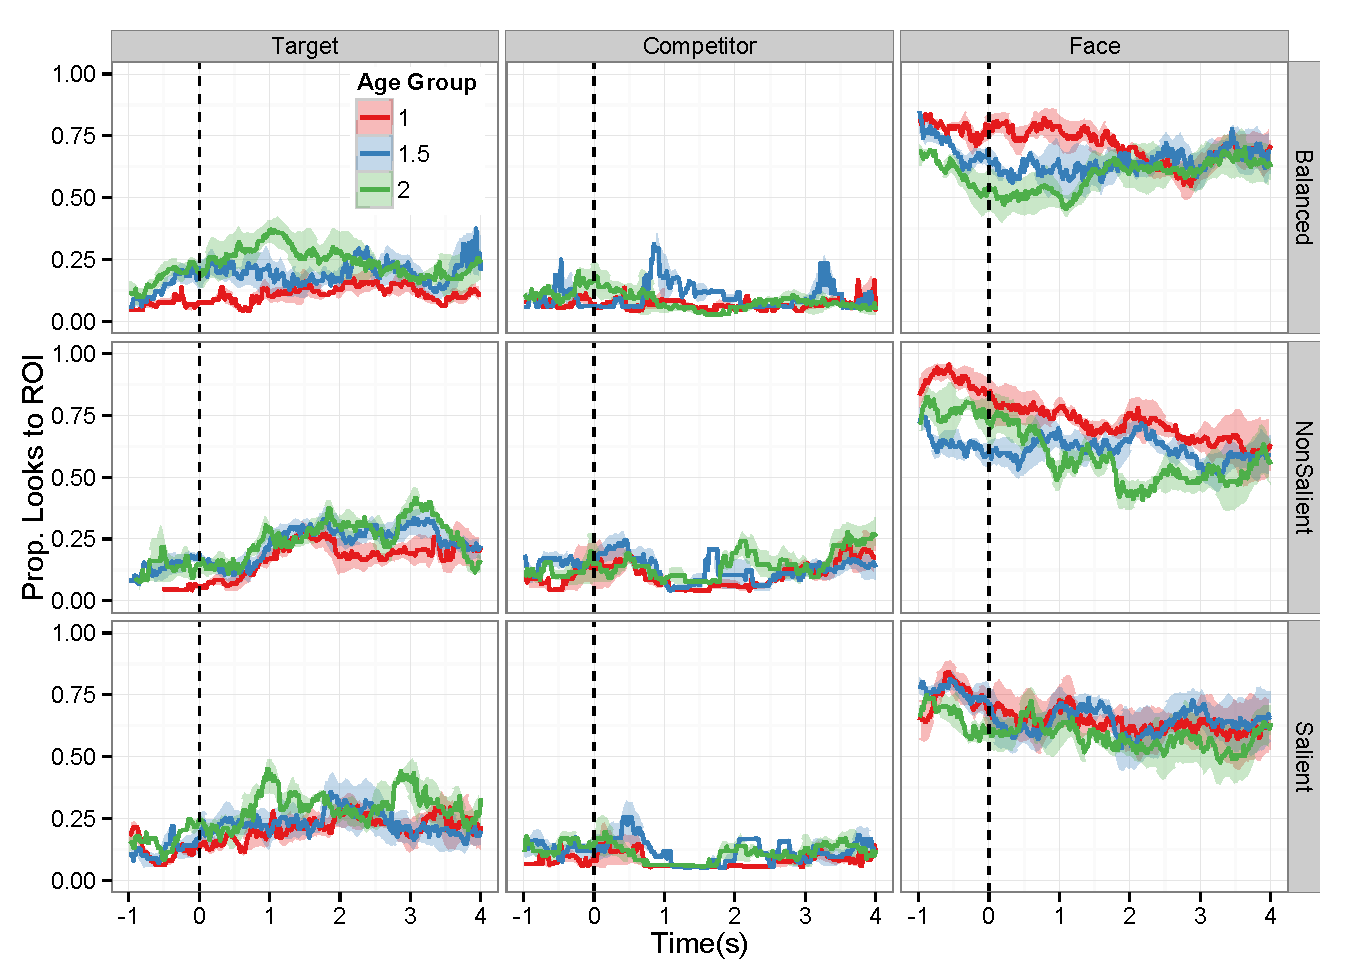
\includegraphics[width=.9\textwidth]{figures/exp1and2_train_spaghetti.pdf}}
	\caption{\label{fig:exp1and2_train_spaghetti} Looking behavior during learning trials in both the Balanced condition of Experiment 1 and the Salient and NonSalient conditions of Experiment 2. In all conditions, children in all age groups were successful in following the speaker's gaze to the target. However, all children also spent the majority of learning trials fixating the speaker's face. Plotting conventions are as in Figure~\ref{fig:exp1_train_spaghetti}}.
\end{figure}

As expected, looking behavior during Familiar test trials was similar across the experiments. Behavior on Novel and ME trials showed a strong effect of condition, however (Figure~\ref{fig:exp1and2_test_spaghetti}). On Novel trials, children in all age groups performed best in the Salient condition, worst in the NonSalient condition, and at an intermediate level in the Balanced condition. That is, children were faster and more accurate at finding the target toy at test when it was the perceptually salient object. In contrast, the Mutual Exclusivity trials showed the opposite pattern: Children in all age groups appeared to succeed in finding the previously-unnamed salient toy when they heard an unfamiliar label, but they had difficulty in the same task when the unnamed toy was not salient. That is, salience appears to have had essentially the same effect on looking behavior regardless of trial type or age: Children were more likely to look at the salient toy.

The effect of salience on looking behavior is even clearer in the onset-contingent analysis (Figure~\ref{fig:exp1and2_split}). Across age groups, area between the target and competitor curves increases for Novel trials in the Salient condition and decreases for the NonSalient condition. Similarly, area increases on ME trials for the NonSalient condition and decreases for the salient condition. 

\begin{figure}[tb]
	\center{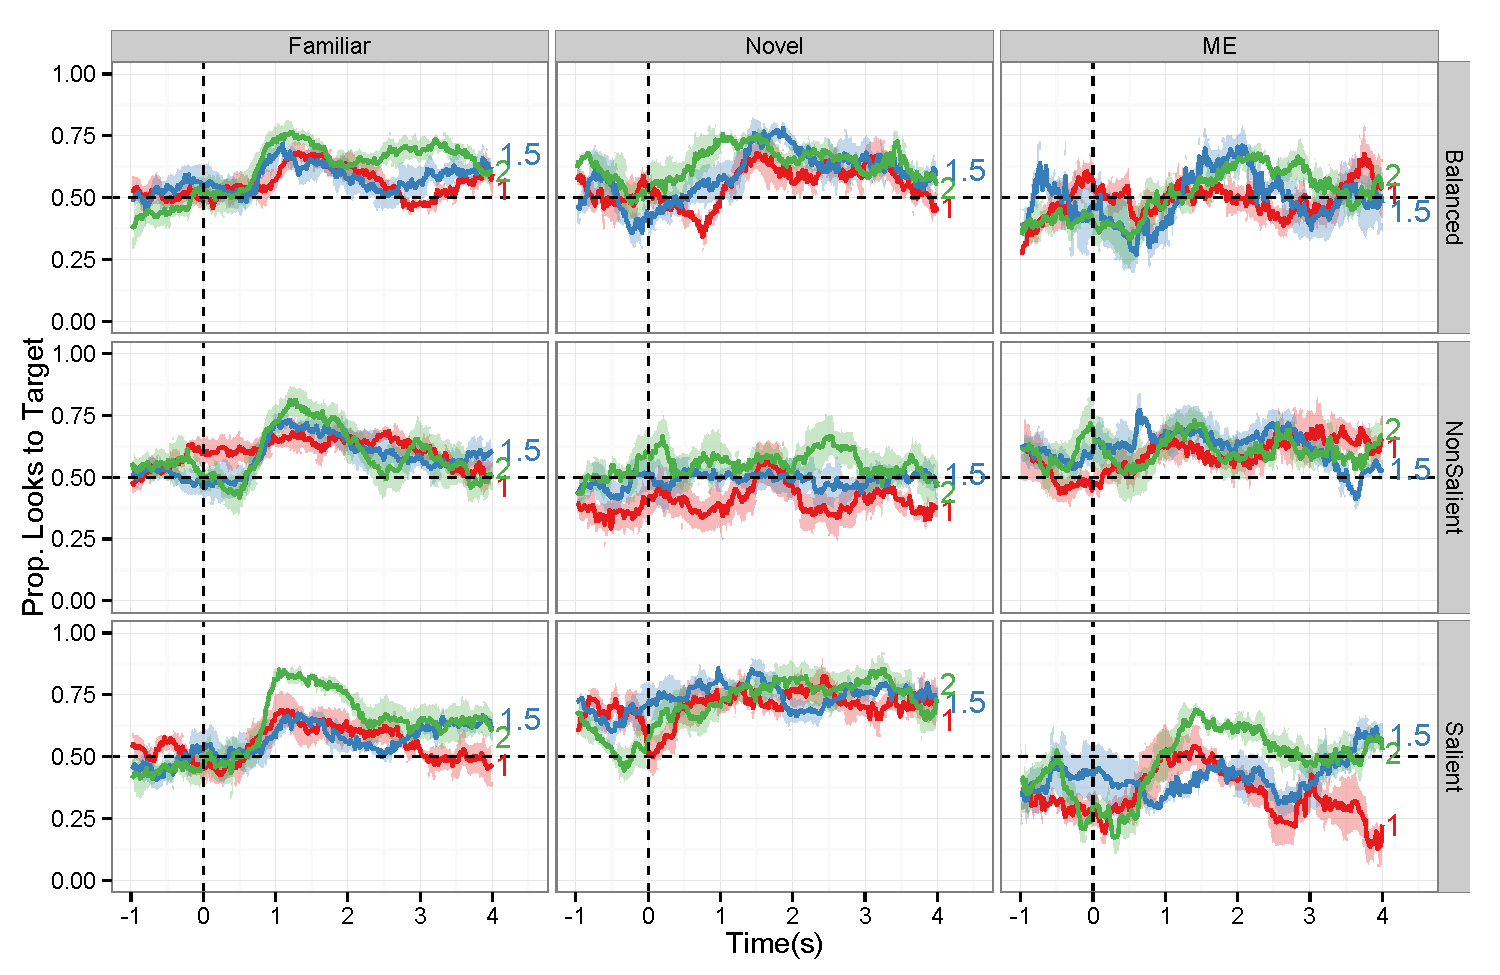
\includegraphics[width=.9\textwidth]{figures/exp1and2_test_spaghetti.pdf}}
	\caption{\label{fig:exp1and2_test_spaghetti} Looking behavior at test in all conditions. In contrast to learning trials, salience had a large effect on looking at test. At all ages, children were drawn to the salient toy regardless of trial type. Plotting conventions are consistent with Figure~\ref{fig:exp1_train_spaghetti}.}
\end{figure}

\begin{figure}[tb]
	\center{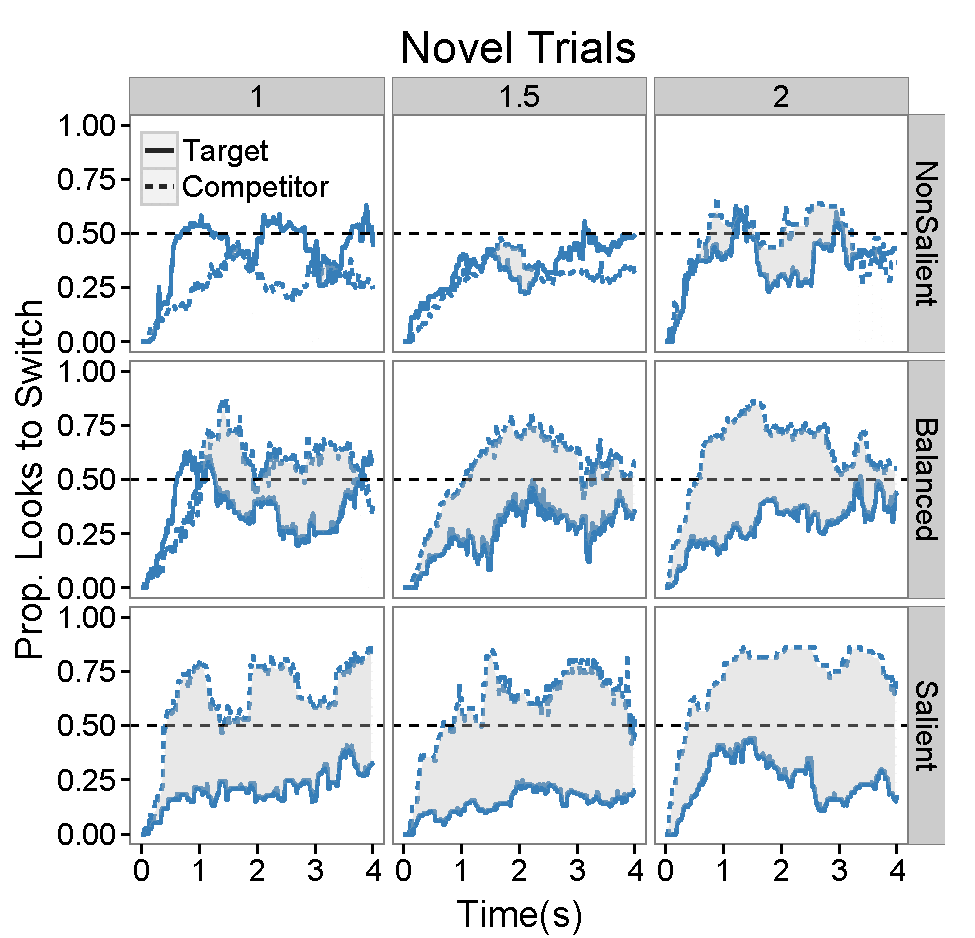
\includegraphics[width=.49\textwidth]{figures/exp1and2_novel_split_plot.pdf}
	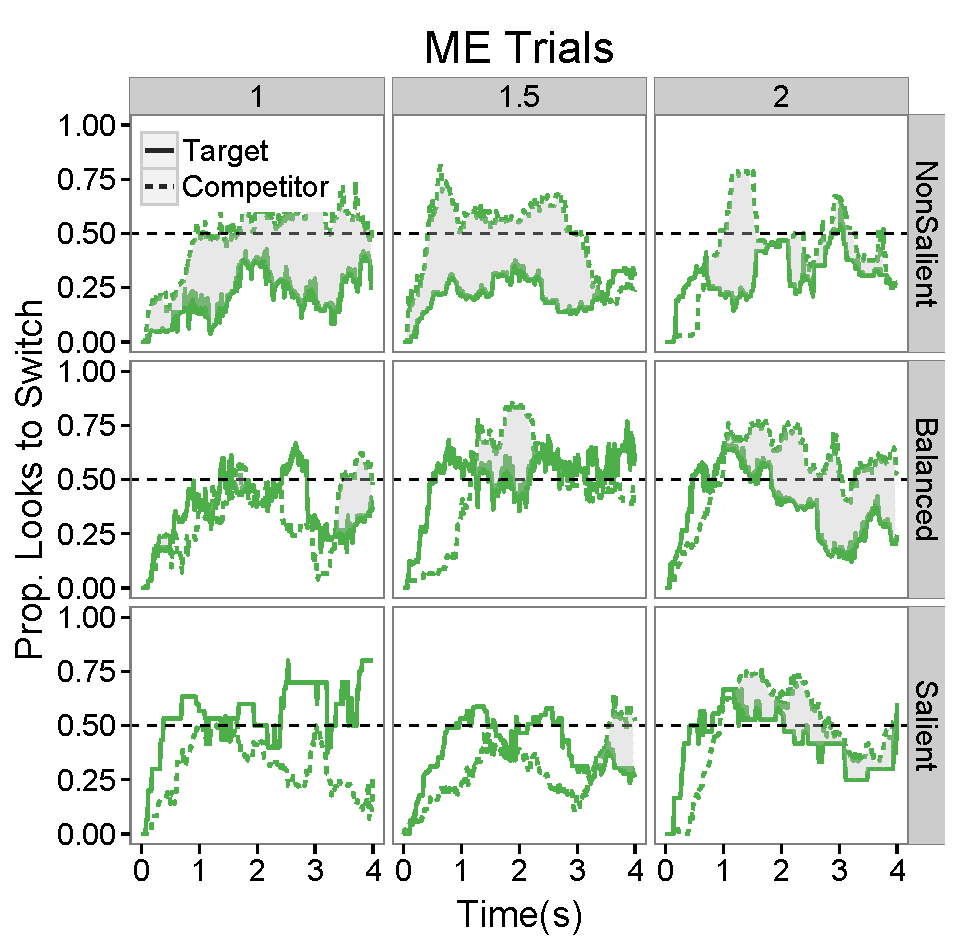
\includegraphics[width=.49\textwidth]{figures/exp1and2_me_split_plot.pdf}}
	\caption{\label{fig:exp1and2_split} Onset-contingent plots for test trials in all conditions. The effect of salience is apparent in comparing the size of the discrimination area for the same trial type across conditions. Areas increased for Novel trials in the Salient condition and decreased in the NonSalient condition. The opposite pattern appears for ME trials. Plotting conventions are consistent with Figure~\ref{fig:exp1_split}.}
\end{figure}

\subsubsection{Statistical Analyses}

In contrast to the prediction of the na\"{i}ve cue-combination account, children's looking behavior during learning trials was not significantly affected by the salience of the target and competitor (Figure~\ref{fig:exp1_2}, top). As in Experiment 1, children of all ages spent more time looking at the target than the competitor (smallest $t(14)  = 3.53$, $p < .01$, $d = 1.32$). Looking time to both target and distractor again made up the minority of their dwell time, however; children spent the majority of learning trials looking at the speaker's face (smallest proportion---2-year-olds in the NonSalient Condition: .51).


\begin{figure}[t]
	\center{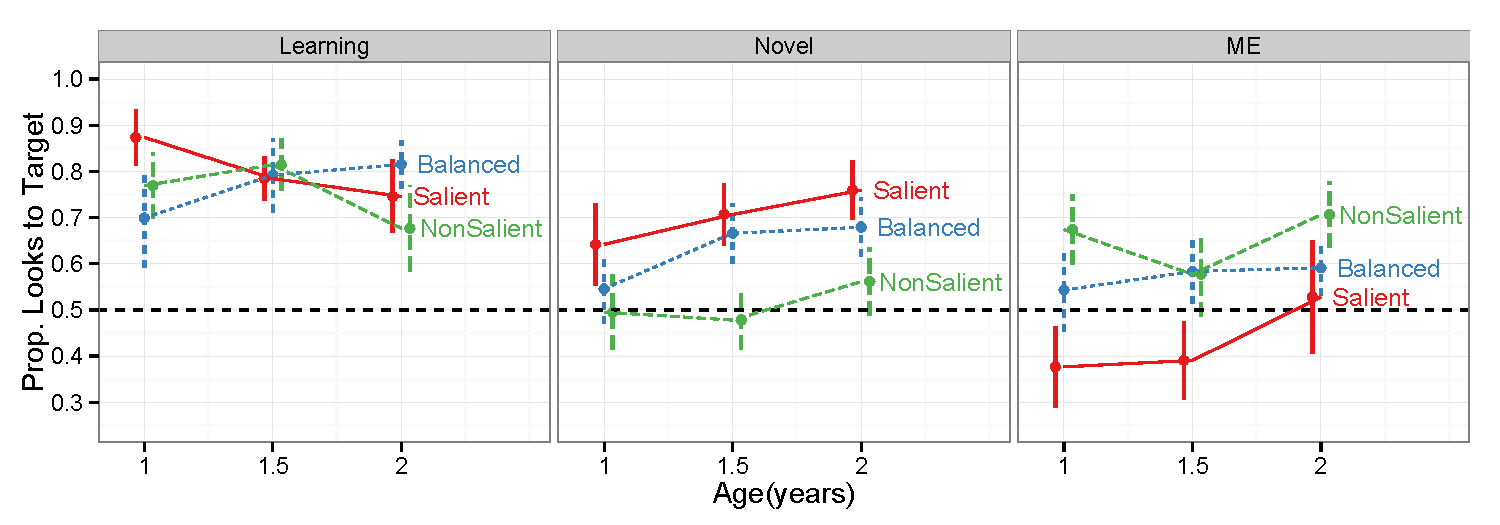
\includegraphics[width=\textwidth]{figures/exp1and2_train_test.pdf}}
	\caption{\label{fig:exp1_2} Proportion of time children fixated the correct target on Learning and Test trials in Experiments 1 (three youngest age groups) and 2. Salience had the predicted effect on looking behavior at test, but relatively little during learning. Each dot indicates one half-year age group and each error bar represents a 95\% confidence interval computed by non-parametric bootstrap. A proportion of .5 indicates chance performance.}
\end{figure}

In principle, this result could be due to the toys being too similar in their salience, making our experiment a weak test of the cue-combination model. But in fact, the differing salience of the two objects exerted a very strong effect during test trials---children in all age groups were strongly attracted to the salient object. When the target referent was salient, children at all ages looked at it for the majority of the window of analysis on Novel test trials (smallest $t(19)  = 2.96$, $p < .01$, $d = .66$). When the target was nonsalient, no age group showed evidence of learning on Novel test trials (largest $t(13)  = 1.46$, $p = .17$, $d = .39$). Mutual Exclusivity (ME) trials showed the opposite pattern. When the target referent was salient, children in the two younger age groups looked at the correct referent on ME trials (the competitor) at \emph{below} chance levels (smallest $t(20) = -2.29$, $p < .05$, $d = .50$). In the NonSalient condition, even the youngest children looked at the correct referent on ME trials at above chance levels (smallest $t(22) = 4.51$, $p < .001$, $d = .94$). Figure~\ref{fig:exp1_2} shows a summary of looking behavior across both Experiments 1 and 2.

The effect of perceptual cues at test did not appear to change across the age range we tested in Experiment 2. We fit a mixed-effects logistic regression to the data from both experiments to determine how age and experimental condition affected looking behavior during both learning and test. After controlling for performance on Familiar trials, this regression showed a significant effect of condition, and an interaction between trial type and condition. Children looked more to the salient object at test regardless of whether it was the target or competitor, and significantly more at the target during learning trials regardless of whether it was salient. No models with additional interactions improved fit to the data, indicating that neither condition nor trial type interacted with age (Table~\ref{tab:model_table}). 

\begin{table}[tb]
\centering
\begin{tabular}{lrrrrl}
 Predictor & Estimate & Std. Error & $z$ value & $p$ value &  \\ 
  \hline
Intercept & -0.63 & 0.63 & -0.99 & 0.32 &  \\ 
  Age(years) & 0.43 & 0.27 & 1.61 & 0.11 &  \\ 
  Familiar & 1.53 & 0.73 & 2.10 & 0.04 & * \\ 
  Salient & 0.92 & 0.48 & 1.90 & 0.06 & . \\ 
  NonSalient & -1.00 & 0.37 & -2.70 & 0.01 & ** \\ 
  Learning & 0.94 & 0.44 & 2.11 & 0.03 & * \\ 
  ME & -0.32 & 0.36 & -0.89 & 0.37 &  \\ 
  Salient $\times$ Learning & 0.00 & 0.84 & 0.00 & 1.00 &  \\ 
  NonSalient $\times$ Learning & 1.15 & 0.65 & 1.76 & 0.08 & . \\ 
  Salient $\times$ ME & -2.23 & 0.61 & -3.65 & 0.00 & *** \\ 
  NonSalient $\times$ ME & 1.59 & 0.54 & 2.92 & 0.00 & ** \\ 
   \hline
\end{tabular}
\vspace{6pt}
\caption{\label{tab:model_table} Mixed-effects logistic regression model for looking behavior in Experiments 1 and 2. The model was specified as \small{\tt{Prop.Correct $\sim$ Age + Condition * TrialType + Familiar + (1 | Subject)}} with the Novel test type in the Balanced Condition as the reference category.}
\end{table}

\subsection{Summary}

These analyses again suggest a model of early word learning different in a number of ways from na\"{i}ve cue combination. First, the perceptual cue had a consistent effect across development, attracting attention similarly for children in all age groups (contra Prediction \#3). Second, this effect was largely absent during learning trials, suggesting that perceptual salience of the target and competitor did not affect children's attention during the naming events (contra Prediction \#4). 

As in Experiment 1, older children in both the Salient and NonSalient condition were better at finding the target on both learning and test trials. But critically, this difference was unrelated to the effect of perceptual salience. Further, after controlling for performance on Familiar test trials, even children's age failed to reach significance as a predictor of looking to the target on learning and test trials. These findings strongly suggest that, although there is clear change in word learning across development, this development is not driven by changing cue weights (Prediction \#1). Instead, the difference appears to derive from changes in other cognitive processes---attention, memory, and language processing.

\section{General Discussion}

Is children's early word-object mapping fundamentally social, or is it mostly driven by perceptual processes? A weighted cue-combination account provides a simple and parsimonious framework to unify social and perceptual factors in early word learning \cite{Hollich2000,Yu2007b,Frank2013a}. Under this kind of account, perceptual cues are weighed higher in early learning, while social cues gradually gain weight as children learn their predictive power across early naming events. We tested this account in two word-learning experiments and found that its predictions were inconsistent with the data. 

Although a na\"{i}ve cue-combination account would predict that developmental change is largely driven by the relative re-weighting of cues, our data showed little evidence of this (contra Prediction \#1). Perceptual salience exerted its effects mostly at test, and did so consistently across early development instead of decreasing in weight (contra Prediction \#2). Social cues appeared to have a differential effect across development, but changes in social cues mirrored increases in familiar word recognition, suggesting that the underlying cause might not be change in cue weight but changes in more general cognitive factors (contra Prediction \#3). Finally, developmental changes during learning appeared to be driven by disengagement from the social stimulus, not disengagement from the perceptually salient competitor object (contra Prediction \#4). 

The  na\"{i}ve cue combination model provides important insights about the different constructs involved in early word learning, but our data nevertheless cause us to reject it as a broader framework for two reasons. First, in consideration of other evidence on early social word learning, we find cue combination to be too impoverished a framework to accommodate the range of communicative inferences that have been shown in young children. Second, na\"{i}ve cue combination fails to provide an adequate account of the developmental changes we observed in our data experimental data.

\paragraph{From cue weighting to communicative inference}

Stepping back from the stripped-down mapping paradigms we studied here, there is a broad literature attesting to the remarkable inferences that early word learners can make on the basis of social evidence. For example, \citeA{Tomasello2000} lists an impressive variety of different inferences from the same limited materials---a speaker's reference in context, modulated by low-level cues like gaze and pointing as well as high-level cues like discourse context or even a speaker's admission of an error. While these inferences are primarily attested with children 18 months and older \cite<e.g.>{Baldwin1993,Akhtar1996}, both observational analyses and looking-time paradigms provide evidence that the same information is present and used in interpretation for even younger children \cite{Frank2013,Vouloumanos2012,Vouloumanos2014}. These findings simply do not admit to an interpretation in terms of a linear combination of cues, whatever their weights. Instead, cues are interpreted depending on their context and the learner's estimation of the speaker's intentions. 

In addition to the issues of applying cue combination to single learning instances, the cue combination framework does not speak to the challenges of interpreting \emph{across} situations. Word learning often relies on processes that work at multiple time-scales. Children need to identify a speaker's referent in-the-moment, encode a mapping between the label and referent, recall multiple labeling events and integrate across them, and use their learned mappings to identify the object in novel contexts \cite{Frank2009a,McMurray2012, Yu2012b}. We have presented data here that falsify some predictions of a na\"ive cue-combination model, but our critiques converge with a broader theoretical problem: na\"{i}ve cue-combination does not distinguish among the component problems that word learners must solve. In our experiments, for instance, children used different cues to identify a speaker's referent and to find it in a novel test context. Building a more satisfying model of the development of word learning will require integrating the cues children use to identify referents with an understanding of how these cues interact with interpretation in the moment. While we do not develop such an account here, we believe that this is a critical next step for theory. 

\paragraph{Domain-general change as an account of developmental differences in word learning}

While other data speak against cue combination as a broader model of social word learning, one attraction of the cue combination model is the clarity of its predictions about the changes the should be observed in word learning across early development, as well as the learning input that should produce these changes. This predictive clarity was the primary rationale for our focus on cue combination in the present studies. Unfortunately, these predictions were not borne out in our data. 

The factors involved in predicting children's responses in our dataset were indeed those identified by cue combination models: both social information and salience played a strong role in determining behavior. But changes in the weights on these cues did not appear to account for our data. At test, perceptual salience was a strong driver even for older children's attention; and during training, social information directed even the youngest children's attention. What changed, however, was whether the children \emph{disengaged} from the social cue, not whether they engaged with it, and whether they \emph{remembered} the mapping that they had learned, not whether they attended to it when it was more salient. 

The nature of children's improvement in identifying the speaker's referent over development cannot be attributed to their learning the predictive validity of gaze as a referential cue. Instead, developmental changes in domain-general cognitive processes appear responsible, although our experiments were not designed to disentangle exactly what these were. Early childhood is a time of substantial development in attention and inhibition \cite{smith1999b,diamond1989}, memory \cite{cowan1997}, and speed of processing \cite{kail1991,dougherty1997}. All of these cognitive processes play a role in our task. Flexible shifting of attention is critical for the learning phase, as is having the inhibitory control to disengage with the face; at test, similarly, the ability to disengage from a more salient competitor image is critical. Memory for the mapping between word and object should play a large part in performance at test as well \cite{Horst2008}. Finally, changes in speed of processing---whether for language specifically or overall---may underly some changes in performance at test, as has been suggested in familiar word processing \cite{fernald1998,fernald2006}. Thus, our findings are congruent with a theoretical model proposed by \citeA{Yu2012b}: Whatever the precise learning mechanisms underlying word-object mapping, these mechanisms must be supported by general processed of attention and memory. Disentangling the roles of these distinct constructs will thus be an important goal for future work. 

\paragraph{Further implications and conclusions}

Despite these differences in interpretation from the cue combination account, our data are not generally inconsistent with the empirical results that motivated previous theory. As observed in previous studies, looking at the target object relative to the competitor object during learning trials increased steadily across development \cite{Moore1999,Hollich2000}. Similarly, novel word learning improved at a similar rate across development. In contrast to previous work, however, we were able to measure children's attention not just to the target and competitor toys, but also to the speaker. Using continuous eye-tracking measures thus gave us additional insight into the dynamics of children's attention and information processing, and ultimately to make different inferences from the data we observed.

In addition to its theoretical consequences, our work here has significant implications for users of two-alternative preferential looking displays. Both \citeA{reznick1990} and \citeA{fernald2008} highlight the importance of matching targets in two-alternative displays. Our work provides further justification for these recommendations. When alternatives were not matched for perceptual salience, the relatively more salient object dominated children's looking preferences for all age groups at test. In particular, we saw evidence of novel word learning for the 1.5--2-year-olds in the balanced salience condition, but this result was masked if the target item was more salient and exaggerated if the target was less salient. This overshadowing-by-salience was, if anything, more pronounced for the mutual exclusivity trials. Especially for young participants, small differences in the perceptual properties of the stimuli may mask learning, presumably because overcoming perceptual salience requires inhibitory control that these young children do not have. 

In sum, early word learning is a fundamentally social process. The virtue of cue combination accounts is that they provide an important decomposition of the broader construct of social context into smaller components that allows for prediction and testing. However, the developmental predictions of such accounts are not supported in our data. Nevertheless, we believe that the kind of tentative synthesis that we have offered here---that social inference must be united with domain-general developmental change---is broadly consistent with the spirit of the Emergentist Coalition Model in its attempt to explain both children's early social inference and the often fragile nature of these inferences as well as their sensitivity to, and sometimes complete moderation by lower-level perceptual processes. Children's social information processing is built from and operates on top of mechanisms for directing their attention, encoding auditory and visual information, retrieving this information later, and combining it across multiple contexts. We propose that the kinds of developmental change in social information processing we observed in our data, and in the data used to motivate cue combination accounts, emerges not from changes in children's cue weights, but instead from developmental changes in these lower-level processes.


\section{Acknowledgments}

We are grateful to Janelle Klaas for collecting the data, to Carissa Romero for help in stimulus creation, and to Molly Lewis and all of the members of the Language and Cognition Lab for their feedback on this project. In addition, we thank the parents, children, and staff at the San Jose Children's Discovery Museum for supporting us in collecting developmental data. This work was supported by NIH NRSA F32HD075577 to DY as well as grants from the Merck Scholars Foundation and the Stanford Center Health Research Initiative to MCF.

\section{Appendix}
\renewcommand\thefigure{A\arabic{figure}}   
\setcounter{figure}{0}    

In order to measure the impact of object salience on children's looking and learning, we needed four distinct objects, two that were equally salient (Balanced 1, Balanced 2), and two that were differentially salient (Salient, NonSalient). We began by estimating the relative salience of a number of different toys using aggregate adult judgments. Thirty-eight adults on Amazon Mechanical Turk were shown two toys at a time from a set of 10. For each pair, they were asked to pick the toy they would rather play with. Each participant made 20 choices, with toys sampled at random, producing $\sim$7.6 responses for each pair of toys. From these responses, we chose two  the two toys that were best balanced against each other as the Balanced toys. Two unbalanced toys were chosen as the Salient and NonSalient toys.

We then validated these relative saliences with a separate sample of children recruited from San Jose Children's Discovery museum. Demographic and experimental data were collected from 33 children, 2 of whom were excluded for failure to calibrate. The final sample consisted of 8 1-2 year olds (3 girls), 8 2-3 year olds (3 girls), 9 3-4 year olds (5 girls), and 6 4-5 year olds (4 girls).

Children were shown each of the four toys used in Experiments 1 and 2, two at a time. Each trial was visually identical to the test trials from the main experiments, but instead of hearing a toy's label, children were only directed by the speaker to ``look!'' Each toy was tested against each other toy twice, once in each possible left-right position. Children's proportion of looking to each toy on each trial was computed, and both trials for each pair were averaged together. Individual trials were dropped from analysis if children did not look at the screen for at least 50\% of their duration.

Proportions of looking for each pair of toys was compared to chance with a one sample t-test. Children showed no significant preferences between any of the toys (largest $t(22) = .80$, $p = .43$, $d =.17$) except for between the Salient and NonSalient toys ($t(22) = 3.66$, $p < .01$, $d =.65$). Figure~\ref{fig:kid_norm} shows mean looking proportions and 95\% confidence intervals for each pairwise comparison. Thus, we can conclude that the Salient toy was indeed more salient than the NonSalient toy to children, and that the two Balanced toys were indeed balanced for object salience.

\begin{figure}[tb]
	\center{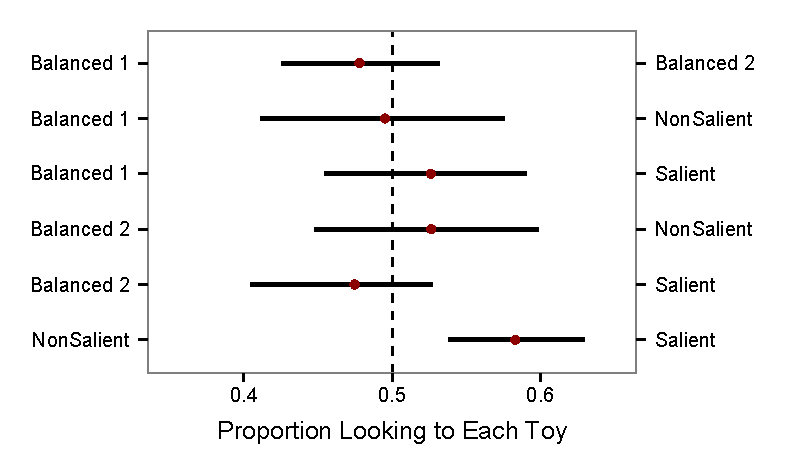
\includegraphics[width=.9\textwidth]{figures/kid_norm.pdf}}
	\caption{\label{fig:kid_norm} Children's preferential looking for all pairwise comparisons between objects in the Norming experiment. Points shows mean proportion of looking, and error bars show 95\% confidence intervals computed by non-parametric bootstrapping. Children showed no pairwise-preferences except for between the Salient and Non Salient toys.}
\end{figure}

\bibliographystyle{apacite}
\bibliography{library12}

\end{document}
